\documentclass{article}
\usepackage{listings}
\usepackage{xcolor}
\usepackage{graphicx}
\usepackage{url}
\usepackage{pdfpages}
\usepackage{makecell}
\usepackage{tabularx}
\usepackage{amsmath}
\usepackage{amssymb}
\usepackage{multirow}
\usepackage{array}

\title{Summary of the Biome Generation in \\ Minecraft 1.8 - 1.12}

\author{Cubitect}

\begin{document}
	
	\maketitle
	
	\begin{abstract}
		This document is designed to provide an overview of how Minecraft biome generation works and how we may efficiently find seeds with desired properties.
	\end{abstract}
	
	\newpage
	
	\tableofcontents
	
	
	
	\newpage
	
	
	\section{Biome Generator Layers}

	Minecraft biome generation occurs in layers. Many of these layers are chained together inside the generator, such that the output from one becomes the input for the next. A flowchart of this can be found on the next page.
	
	Each layer applies certain modifications to a map of integers, which change their use throughout the generation process. Initially the map only contains values 0 or 1, representing ocean or land masses. Later in the generator they represent temperature categories, until they are finally replaced by the actual biome IDs.
	
	Some of the layers resize the output of the previous layer. These Zoom-layers therefore change how much area is represented by a map entry. I will refer to this as "scale". For instance, 1:256 should be read as: one map entry ends up as an area of 256x256 blocks in the world.
	
	\setcounter{subsection}{-1}
	\subsection{Seed Finding}
	
	When constructing a seed finder, it may be useful to stop the generation at an earlier layer. For example if we require a swamp to be located near a given position, then we might want to generate up to layer 19: Biome first, and then check on a 1:256 scale if there is a swamp in the area. This is not enough to confirm that there will be a swamp at the given position, but we can rule out seeds that definitely don't have a swamp anywhere near the area. If the seed passes this cheap test, then we can go through the full expensive generation process and directly check the position for a swamp.
	
	Usually it is not practical to continue the search from a terminated generation and we have to start over again. The reason for this is that most layers require an additional 1 wide boarder from the previous layer, so the map sizes don't match up.
	
	Another more involved, but very powerful way of creating early knock-out criteria is to check if there is a some condition in the layer chain that is independent of the rest of the biomes. For instance in the case of finding a swamp, we can notice that there is a pseudo-random number check in layer 19: Biome, that converts Lush temperature climates to swamplands. However, the pseudo-random number generator is seeded by a combination of the position and the world seed, so we can make sure the random number output gives the required value without going through the rest of the layers. The more expensive generator can afterwards be used to make sure that a Lush climate is actually present at that position.
	
	
	In the summary below in sections 1.1 -- 1.44 I have laid out some of the properties of each layer, such as the scale of the layer and the possible values for the map entries with their respective average probability of occurrence (Note: these are estimates and may vary). When constructing a seed finder these values can be used as a reference to determine reasonable cut-off points for the generator.
	
	
	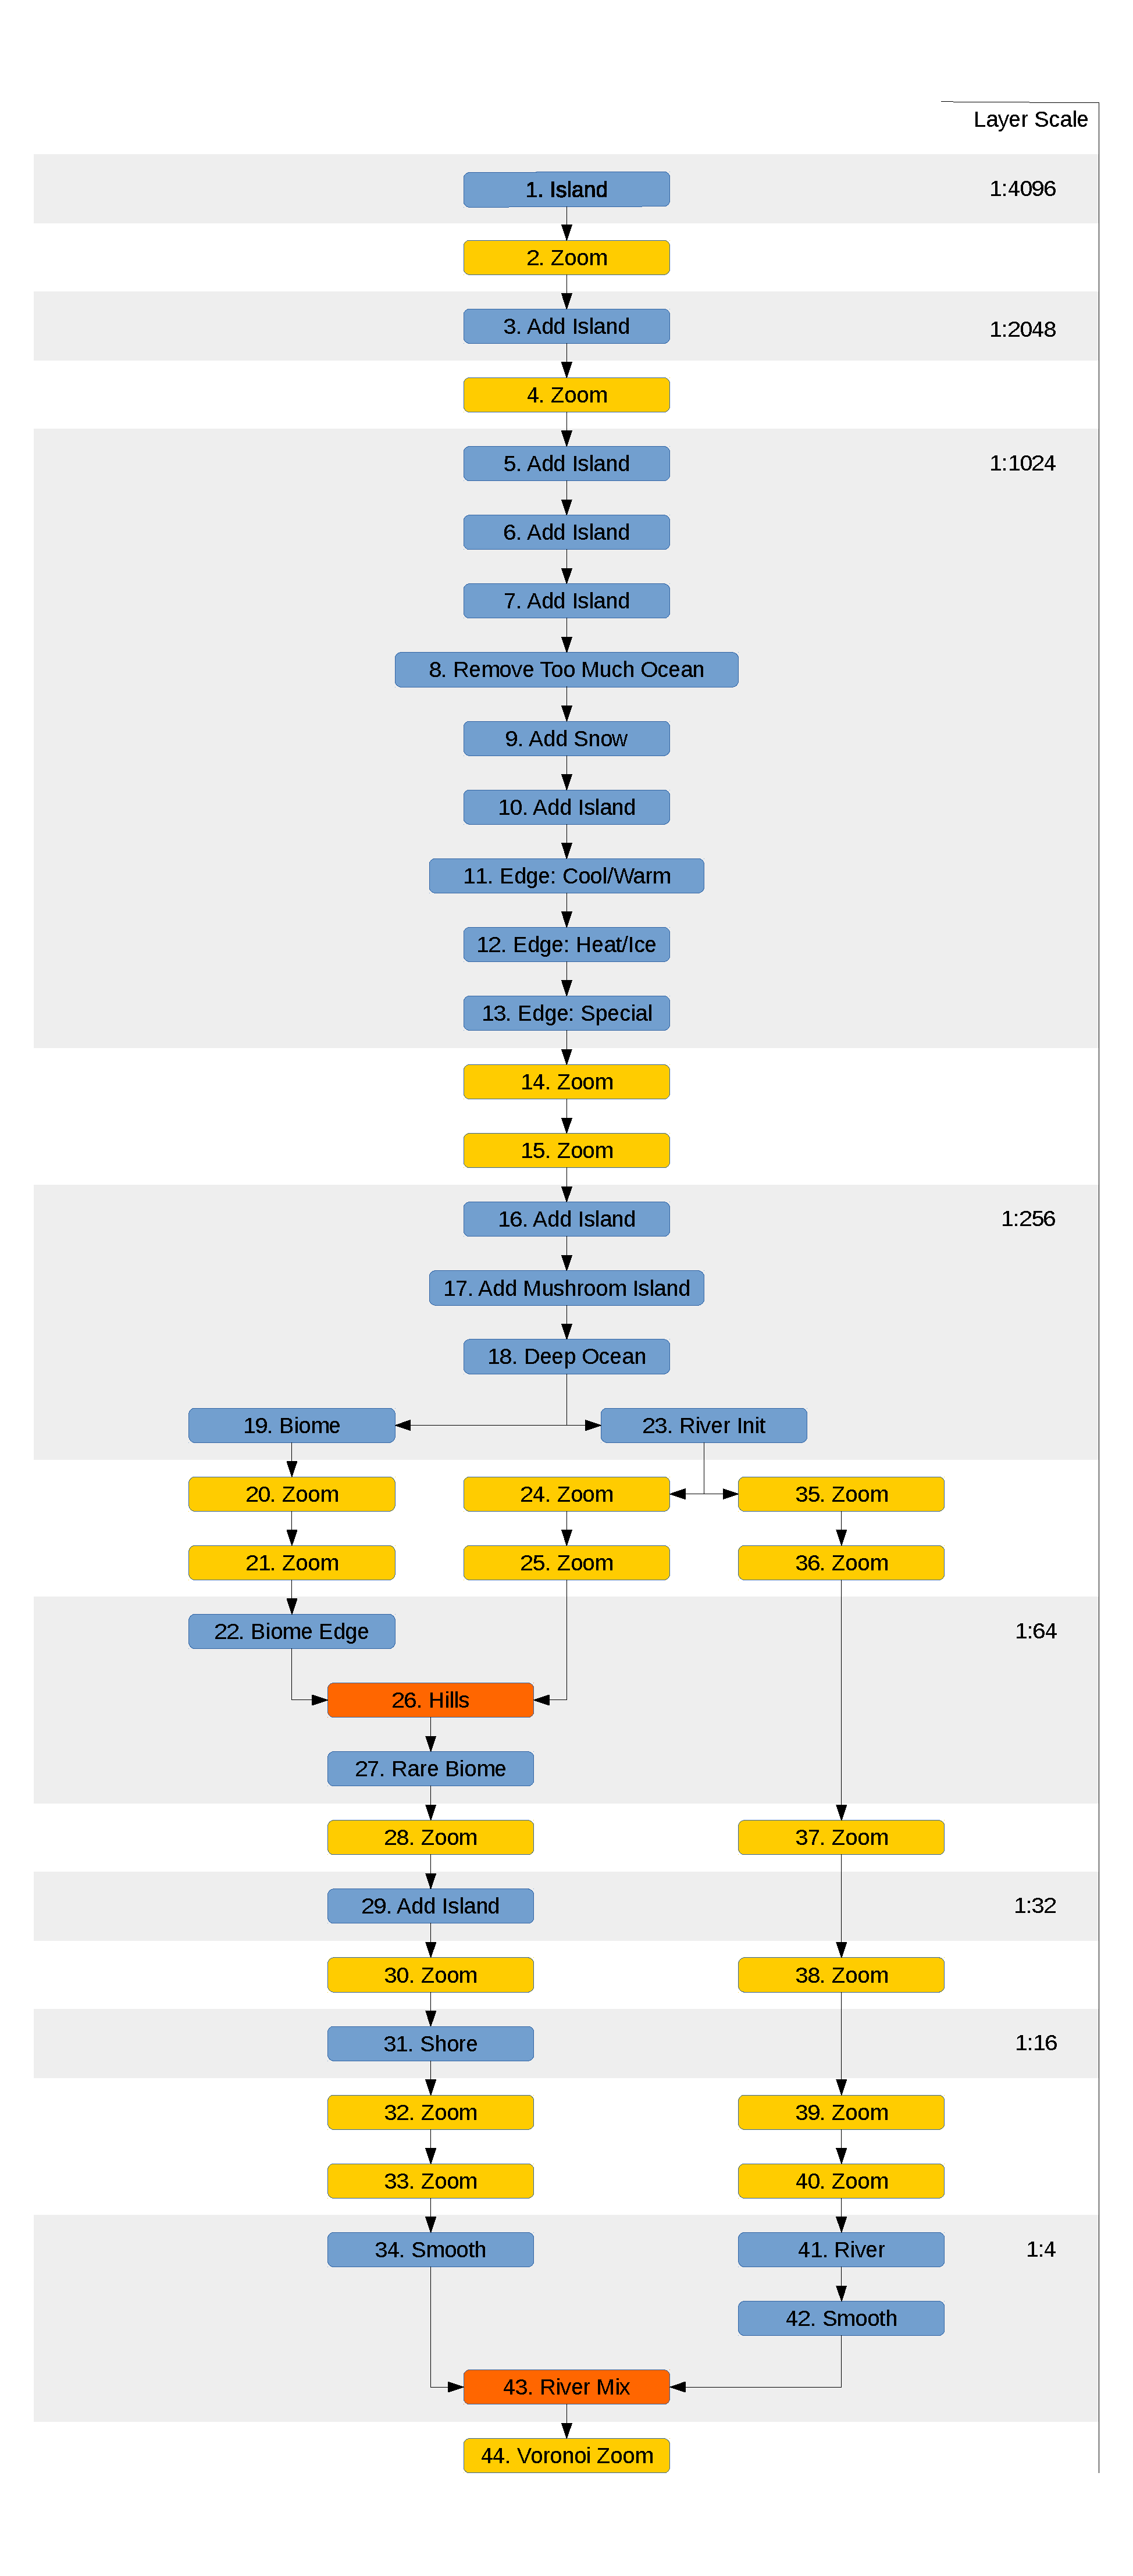
\includepdf[pages={1}]{layers.pdf}
	
	
	\subsection{Layer 1: Island}
	\begin{tabular}{|l|l|l|}\hline
		Scale: & \multicolumn{2}{|l|}{1:4096} \\\hline\hline
		Value  & Type   & Occurrence \\\hline
		0      & Ocean  & 90.0\%\\\hline
		1      & Land   & 10.0\%\\\hline
	\end{tabular}
	
	\subsection{Layer 2: Zoom}
	\begin{tabular}{|l|l|l|}\hline
		Scale: & \multicolumn{2}{|l|}{1:2048} \\\hline\hline
		Value  & Type   & Occurrence \\\hline
		0      & Ocean  & 90.0\%\\\hline
		1      & Land   & 10.0\%\\\hline
	\end{tabular}
	
	\subsection{Layer 3: Add Island}
	\begin{tabular}{|l|l|l|}\hline
		Scale: & \multicolumn{2}{|l|}{1:2048} \\\hline\hline
		Value  & Type   & Occurrence \\\hline
		0      & Ocean  & 84.3\%\\\hline
		1      & Land   & 15.7\%\\\hline
	\end{tabular}

	\subsection{Layer 4: Zoom}
	\begin{tabular}{|l|l|l|}\hline
		Scale: & \multicolumn{2}{|l|}{1:1024} \\\hline\hline
		Value  & Type   & Occurrence \\\hline
		0      & Ocean  & 84.9\%\\\hline
		1      & Land   & 15.1\%\\\hline
	\end{tabular}
	
	\subsection{Layer 5: Add Island}
	\begin{tabular}{|l|l|l|}\hline
		Scale: & \multicolumn{2}{|l|}{1:1024} \\\hline\hline
		Value  & Type   & Occurrence \\\hline
		0      & Ocean  & 81.4\%\\\hline
		1      & Land   & 18.6\%\\\hline
	\end{tabular}
	
	\subsection{Layer 6: Add Island}
	\begin{tabular}{|l|l|l|}\hline
		Scale: & \multicolumn{2}{|l|}{1:1024} \\\hline\hline
		Value  & Type   & Occurrence \\\hline
		0      & Ocean  & 77.5\%\\\hline
		1      & Land   & 22.5\%\\\hline
	\end{tabular}
	
	\subsection{Layer 7: Add Island}
	\begin{tabular}{|l|l|l|}\hline
		Scale: & \multicolumn{2}{|l|}{1:1024} \\\hline\hline
		Value  & Type   & Occurrence \\\hline
		0      & Ocean  & 73.4\%\\\hline
		1      & Land   & 26.6\%\\\hline
	\end{tabular}

	\subsection{Layer 8: Remove Too Much Ocean}
	\begin{tabular}{|l|l|l|}\hline
		Scale: & \multicolumn{2}{|l|}{1:1024} \\\hline\hline
		Value  & Type   & Occurrence \\\hline
		0      & Ocean  & 49.4\%\\\hline
		1      & Land   & 50.6\%\\\hline
	\end{tabular}
	
	
	\subsection{Layer 9: Add Snow}
	\begin{tabular}{|l|l|l|}\hline
		Scale: & \multicolumn{2}{|l|}{1:1024} \\\hline\hline
		Value  & Type     & Occurrence \\\hline
		0      & Ocean    & 49.4\%\\\hline
		1      & Warm     & 33.7\%\\\hline
		3      & Cold     & 4.8\%\\\hline
		4      & Freezing & 12.4\%\\\hline
	\end{tabular}
	
	\medskip\noindent
	Changes some of the land starting points to Cold and Freezing.

	\subsection{Layer 10: Add Island}
	\begin{tabular}{|l|l|l|}\hline
		Scale: & \multicolumn{2}{|l|}{1:1024} \\\hline\hline
		Value  & Type    & Occurrence \\\hline
		0      & Ocean   & 33.8\%\\\hline
		1      & Warm    & 37.6\%\\\hline
		3      & Cold    & 4.8\%\\\hline
		4      & Freeing & 23.9\%\\\hline
	\end{tabular}
	
	\medskip\noindent
	Spreads out the continental areas, decreasing the amount of ocean.

	\subsection{Layer 11: Edge, Cool/Warm}
	\begin{tabular}{|l|l|l|}\hline
		Scale: & \multicolumn{2}{|l|}{1:1024} \\\hline\hline
		Value  & Type     & Occurrence \\\hline
		0      & Ocean    & 33.8\%\\\hline
		1      & Warm     & 13.6\%\\\hline
		2      & Lush     & 23.9\%\\\hline
		3      & Cold     & 4.8\%\\\hline
		4      & Freezing & 23.9\%\\\hline
	\end{tabular}
	
	\medskip\noindent
	Changes Warm(1) lands which are adjacent to Cold(3) or Freezing(4) temperatures to Lush(2).
	
	\subsection{Layer 12: Edge, Heat/Ice}
	\begin{tabular}{|l|l|l|}\hline
		Scale: & \multicolumn{2}{|l|}{1:1024} \\\hline\hline
		Value  & Type     & Occurrence \\\hline
		0      & Ocean    & 33.8\%\\\hline
		1      & Warm     & 13.6\%\\\hline
		2      & Lush     & 23.9\%\\\hline
		3      & Cold     & 23.9\%\\\hline
		4      & Freezing & 4.8\%\\\hline
	\end{tabular}

	\medskip\noindent
	Changes Freezing(4) lands which are adjacent to Warm(1) or Lush(2) temperatures to Cold(3).

	\subsection{Layer 13: Edge, Special}
	\begin{tabular}{|l|l|l|}\hline
		Scale: & \multicolumn{2}{|l|}{1:1024} \\\hline\hline
		Value  & Type     & Occurrence \\\hline
		0      & Ocean    & 33.8\%\\\hline
		1      & Warm     & 12.5\%\\\hline
		2      & Lush     & 22.1\%\\\hline
		3      & Cold     & 22.1\%\\\hline
		4      & Freezing & 4.4\%\\\hline
		-      & Special  & 5.1\% / 60\\\hline
	\end{tabular}
	
	\medskip\noindent
	Marks every 1 in 13 lands (non-ocean) as special, by adding a 4-bit number in 0x0F00 to the value.
	
	
	\subsection{Layer 14: Zoom}
	\begin{tabular}{|l|l|l|}\hline
		Scale: & \multicolumn{2}{|l|}{1:512} \\\hline\hline
		Value  & Type   & Occurrence \\\hline
		0      & Ocean    & 35.6\%\\\hline
		1      & Warm     & 12.2\%\\\hline
		2      & Lush     & 21.9\%\\\hline
		3      & Cold     & 21.9\%\\\hline
		4      & Freezing & 4.2\%\\\hline
		-      & Special  & 4.2\% / 60\\\hline
	\end{tabular}

	\subsection{Layer 15: Zoom}
	\begin{tabular}{|l|l|l|}\hline
		Scale: & \multicolumn{2}{|l|}{1:256} \\\hline\hline
		Value  & Type   & Occurrence \\\hline
		0      & Ocean    & 35.6\%\\\hline
		1      & Warm     & 11.9\%\\\hline
		2      & Lush     & 21.9\%\\\hline
		3      & Cold     & 21.9\%\\\hline
		4      & Freezing & 4.2\%\\\hline
		-      & Special  & 4.5\% / 60\\\hline
	\end{tabular}
	
	\subsection{Layer 16: Add Island}
	\begin{tabular}{|l|l|l|}\hline
		Scale: & \multicolumn{2}{|l|}{1:256} \\\hline\hline
		Value  & Type   & Occurrence \\\hline
		0      & Ocean    & 31.4\%\\\hline
		1      & Warm     & 12.7\%\\\hline
		2      & Lush     & 22.4\%\\\hline
		3      & Cold     & 22.8\%\\\hline
		4      & Freezing & 6.2\%\\\hline
		-      & Special  & 4.5\% / 60\\\hline
	\end{tabular}
	
	
	\subsection{Layer 17: Add Mushroom Island}
	\begin{tabular}{|l|l|l|l|}\hline
		Scale: & \multicolumn{3}{|l|}{1:256} \\\hline\hline
		Value  & Type     & \multicolumn{2}{l|}{Occurrence} \\\hline
		0      & Ocean    & \multicolumn{2}{l|}{31.4\%}\\\hline
		1      & Warm     & \multicolumn{2}{l|}{12.8\%}\\\hline
		2      & Lush     & \multicolumn{2}{l|}{22.5\%}\\\hline
		3      & Cold     & \multicolumn{2}{l|}{22.7\%}\\\hline
		4      & Freezing & \multicolumn{2}{l|}{6.08\%}\\\hline
		14     & Mushroom & \multicolumn{2}{l|}{0.0773\%}\\\hline\hline
		
		\makecell[l]{ $(n<<8)+1$ \\ with $n = $ \\ $1, 4, 7, 10, 13$ } & - & 
		\makecell[l]{0.0690\% \\each} & \multirow{5}{*}{0.90\%}\\\cline{1-3}
		
		\makecell[l]{ $(n<<8)+1$ \\ with $n = $ \\ $2, 3, 5, 6, 8, 9,$ \\ $11, 12, 14, 15$ } & - & \makecell[l]{0.0553\% \\ each} & \\\hline\hline
		
		\makecell[l]{ $(n<<8)+2$ \\ with $n = $ \\ $1, 4, 7, 10, 13$ } & - & 
		\makecell[l]{0.1236\% \\ each} & \multirow{5}{*}{1.56\%}\\\cline{1-3}
		
		\makecell[l]{ $(n<<8)+2$ \\ with $n = $ \\ $2, 3, 5, 6, 8, 9,$ \\ $11, 12, 14, 15$ } & - & \makecell[l]{0.0961\% \\ each} & \\\hline\hline
		
		\makecell[l]{ $(n<<8)+3$ \\ with $n = $ \\ $1, 4, 7, 10, 13$ } & - & 
		\makecell[l]{0.1078\% \\ each} & \multirow{5}{*}{1.58\%}\\\cline{1-3}
		
		\makecell[l]{ $(n<<8)+3$ \\ with $n = $ \\ $2, 3, 5, 6, 8, 9,$ \\ $11, 12, 14, 15$ } & - &
		\makecell[l]{0.1037\% \\ each} & \\\hline\hline
				
		\makecell[l]{ $(n<<8)+4$ \\ with $n = $ \\ $1, 4, 7, 10, 13$ } & - & 
		\makecell[l]{0.0212\% \\ each} & \multirow{5}{*}{0.32\%}\\\cline{1-3}
		
		\makecell[l]{ $(n<<8)+4$ \\ with $n = $ \\ $2, 3, 5, 6, 8, 9,$ \\ $11, 12, 14, 15$ } & - &
		\makecell[l]{0.0212\% \\ each} & \\\hline

	\end{tabular}
	
	\medskip\noindent
	Changes every 100th Ocean (adjacent to more Ocean) to Mushroom Island. The special land types are written out in full in the table above. (Note "$<<$" represents a left bit shit.) Added together, the special types make up an average of about 4.37\% of the area.
	
	
	\subsection{Layer 18: Deep Ocean}
	\begin{tabular}{|l|l|l|}\hline
		Scale: & \multicolumn{2}{|l|}{1:256} \\\hline\hline
		Value  & Type       & Occurrence \\\hline
		0      & Ocean      & 22.0\%\\\hline
		1      & Warm       & 12.8\%\\\hline
		2      & Lush       & 22.5\%\\\hline
		3      & Cold       & 22.7\%\\\hline
		4      & Freezing   & 6.1\%\\\hline
		14     & Mushroom   & 0.0773\%\\\hline
		24     & Deep Ocean & 9.4\%\\\hline
		-      & Special    & 4.4\% / 60\\\hline
	\end{tabular}
	
	\medskip\noindent
	Changes any Ocean which is surrounded by more Ocean to Deep Ocean.\\
	(Special lands still have the same statistics as shown for Layer 17.)
	
	
	\subsection{Layer 19: Biome}
	\begin{tabular}{|l|l|l|}\hline
		Scale: & \multicolumn{2}{|l|}{1:256} \\\hline\hline
		Value  & Type           & Occurrence \\\hline
		0      & ocean          & 22.0\%\\\hline
		1      & plains         & 11.6\%\\\hline
		2      & desert         & 6.41\%\\\hline
		3      & extremeHills   & 9.44\%\\\hline
		4      & forest         & 9.43\%\\\hline
		5      & taiga          & 5.68\%\\\hline
		6      & swampland      & 3.75\%\\\hline
		12     & icePlains      & 4.80\%\\\hline
		14     & mushroomIsland & 0.0773\%\\\hline
		21     & jungle         & 1.58\%\\\hline
		24     & deepOcean      & 9.38\%\\\hline
		27     & birchForest    & 3.75\%\\\hline
		29     & roofedForest   & 3.75\%\\\hline
		30     & coldTaiga      & 1.60\%\\\hline
		32     & megaTaiga      & 1.58\%\\\hline
		35     & savanna        & 4.28\%\\\hline
		38     & mesaPlateau\_F & 0.598\%\\\hline
		39     & mesaPlateau    & 0.299\%\\\hline
	\end{tabular}

	\medskip\noindent
	Assigns the actual biome IDs to the lands, based on the temperature category of the land. To be more specific the selection criteria are: 
	
	\begin{tabular}{l c c l}
	
	Temperature & & Weight & Biome \\\hline\hline
	
	Warm & $\longrightarrow$ & 
	\makecell[c]{1/2 \\ 1/3 \\ 1/6} &
	\makecell[l]{desert \\ savanna \\ plains} \\\hline
	
	Warm, special & $\longrightarrow$ &
	\makecell[c]{1/3 \\ 2/3} &
	\makecell[l]{mesaPlateau \\ mesaPlateau\_F} \\\hline
	
	Lush & $\longrightarrow$ & 
	\makecell[c]{1/6 \\ 1/6 \\ 1/6 \\ 1/6 \\ 1/6 \\ 1/6} &
	\makecell[l]{forest \\ roofedForest \\ extremeHills \\ plains \\ birchForest \\ swampland} \\\hline
	
	Lush, special & $\longrightarrow$ & 
	\makecell[c]{1/1} &
	jungle \\\hline

	Cold & $\longrightarrow$ & 
	\makecell[c]{1/4 \\ 1/4 \\ 1/4 \\ 1/4} &
	\makecell[l]{forest \\ extremeHills \\ taiga \\ plains} \\\hline
	
	Cold, special & $\longrightarrow$ & 
	\makecell[c]{1/1} &
	megaTaiga \\\hline
	
	Freezing& $\longrightarrow$ & 
	\makecell[c]{3/4 \\ 1/4} & 
	\makecell[l]{icePlains \\ coldTaiga}
	
	\end{tabular}
	
	\medskip\noindent
	Ocean and Mushroom types are not affected by this layer. The special category is selected when one of the higher bits (0xF00) are set. E.g. 0x603 has high bits and is thus a special Cold(3) category.
	
	
	\subsection{Layer 20: Zoom}
	\begin{tabular}{|l|l|l|}\hline
		Scale: & \multicolumn{2}{|l|}{1:128} \\\hline\hline
		Value  & Type           & Occurrence \\\hline
		0      & ocean          & 23.6\%\\\hline
		1      & plains         & 11.3\%\\\hline
		2      & desert         & 6.48\%\\\hline
		3      & extremeHills   & 9.28\%\\\hline
		4      & forest         & 9.28\%\\\hline
		5      & taiga          & 5.52\%\\\hline
		6      & swampland      & 3.61\%\\\hline
		12     & icePlains      & 4.94\%\\\hline
		14     & mushroomIsland & 0.0586\%\\\hline
		21     & jungle         & 1.62\%\\\hline
		24     & deepOcean      & 9.09\%\\\hline
		27     & birchForest    & 3.61\%\\\hline
		29     & roofedForest   & 3.61\%\\\hline
		30     & coldTaiga      & 1.45\%\\\hline
		32     & megaTaiga      & 1.62\%\\\hline
		35     & savanna        & 4.12\%\\\hline
		38     & mesaPlateau\_F & 0.602\%\\\hline
		39     & mesaPlateau    & 0.279\%\\\hline
	\end{tabular}

	
	\subsection{Layer 21: Zoom}
	\begin{tabular}{|l|l|l|}\hline
		Scale: & \multicolumn{2}{|l|}{1:64} \\\hline\hline
		Value  & Type           & Occurrence \\\hline
		0      & ocean          & 23.9\%\\\hline
		1      & plains         & 11.2\%\\\hline
		2      & desert         & 6.50\%\\\hline
		3      & extremeHills   & 9.23\%\\\hline
		4      & forest         & 9.23\%\\\hline
		5      & taiga          & 5.49\%\\\hline
		6      & swampland      & 3.56\%\\\hline
		12     & icePlains      & 5.00\%\\\hline
		14     & mushroomIsland & 0.0543\%\\\hline
		21     & jungle         & 1.62\%\\\hline
		24     & deepOcean      & 9.03\%\\\hline
		27     & birchForest    & 3.58\%\\\hline
		29     & roofedForest   & 3.57\%\\\hline
		30     & coldTaiga      & 1.43\%\\\hline
		32     & megaTaiga      & 1.62\%\\\hline
		35     & savanna        & 4.08\%\\\hline
		38     & mesaPlateau\_F & 0.603\%\\\hline
		39     & mesaPlateau    & 0.275\%\\\hline
	\end{tabular}
	\subsection{Layer 22: Biome Edge}
	\begin{tabular}{|l|l|l|}\hline
		Scale: & \multicolumn{2}{|l|}{1:64} \\\hline\hline
		Value  & Type             & Occurrence \\\hline
		0      & ocean            & 23.9\%\\\hline
		1      & plains           & 11.2\%\\\hline
		2      & desert           & 6.48\%\\\hline
		3      & extremeHills     & 9.23\%\\\hline
		4      & forest           & 9.23\%\\\hline
		5      & taiga            & 6.01\%\\\hline
		6      & swampland        & 3.47\%\\\hline
		12     & icePlains        & 5.00\%\\\hline
		14     & mushroomIsland   & 0.0543\%\\\hline
		21     & jungle           & 1.62\%\\\hline
		23     & jungleEdge       & 0.0144\%\\\hline
		24     & deepOcean        & 9.03\%\\\hline
		27     & birchForest      & 3.58\%\\\hline
		29     & roofedForest     & 3.57\%\\\hline
		30     & coldTaiga        & 1.43\%\\\hline
		32     & megaTaiga        & 1.11\%\\\hline
		34     & extremeHillsPlus & 0.0111\%\\\hline
		35     & savanna          & 4.09\%\\\hline
		37     & mesa             & 0.321\%\\\hline
 		38     & mesaPlateau\_F   & 0.385\%\\\hline
		39     & mesaPlateau      & 0.172\%\\\hline
	\end{tabular}
	
	\medskip\noindent
	Introduces the biomes jungleEdge, extremeHillsPlus and mesa. The conditional biome changes that take place in this layer are:
	
	\begin{tabular}{l c l}
		mesaPlateau\_F & $\longrightarrow$ & mesa\\
		mesaPlateau & $\longrightarrow$ & mesa\\
		megaTaiga & $\longrightarrow$ & taiga\\
		desert & $\longrightarrow$ & extremeHillsPlus\\
		swampland & $\longrightarrow$ & jungleEdge \\
		swampland & $\longrightarrow$ & plains
	\end{tabular}

	\subsection{Layer 23: River Init}
	
	Starts a new branch of off Layer 18: Deep Ocean. This layer overwrites each map entry that is not Ocean(0) with a pseudo random number between 2 and 300000 (inclusive).
	
	\subsection{Layer 24: Zoom}
	\subsection{Layer 25: Zoom}
	
	\subsection{Layer 26: Hills}
	This is a multilayer which joins the biome generation with the river generator branch at the layers Biome Edge (22) and Zoom (25). However at this stage the river branch is mostly just used as a pseudo random number source. 
	
	\medskip\noindent
	\begin{tabular}{|l|l|l|}\hline
		Scale: & \multicolumn{2}{|l|}{1:64} \\\hline\hline
		Value  & Type             & Occurrence \\\hline
		0      & ocean            & 17.5\%\\\hline
		1      & plains           & 9.86\%\\\hline
		2      & desert           & 4.83\%\\\hline
		3      & extremeHills     & 6.95\%\\\hline
		4      & forest           & 8.87\%\\\hline
		5      & taiga            & 4.67\%\\\hline
		6      & swampland        & 3.36\%\\\hline
		12     & icePlains        & 3.54\%\\\hline
		13     & iceMountains     & 1.30\%\\\hline
		14     & mushroomIsland   & 0.0543\%\\\hline
		17     & desertHills      & 1.46\%\\\hline
		18     & forestHills      & 2.68\%\\\hline
		19     & taigaHills       & 1.15\%\\\hline
		21     & jungle           & 1.15\%\\\hline
		22     & jungleHills      & 0.420\%\\\hline
		23     & jungleEdge       & 0.0140\%\\\hline
		24     & deepOcean        & 14.4\%\\\hline
		27     & birchForest      & 2.58\%\\\hline
		28     & birchForestHills & 0.800\%\\\hline
		29     & roofedForest     & 2.57\%\\\hline
		30     & coldTaiga        & 1.11\%\\\hline
		31     & coldTaigaHills   & 0.282\%\\\hline
		32     & megaTaiga        & 0.688\%\\\hline
		33     & megaTaigaHills   & 0.344\%\\\hline
		34     & extremeHillsPlus & 1.80\%\\\hline
		35     & savanna          & 3.05\%\\\hline
		36     & savannaPlateau   & 0.830\%\\\hline
		37     & mesa             & 0.486\%\\\hline
		38     & mesaPlateau\_F   & 0.240\%\\\hline
		39     & mesaPlateau      & 0.107\%\\\hline
	\end{tabular}
	\newpage\noindent
	\begin{tabular}{|l|l|l|}\hline
		129    & Sunflower Plains     & 0.4816\%\\\hline
		130    & Desert M             & 0.1971\%\\\hline
		131    & Extreme Hills M      & 0.2944\%\\\hline
		132    & Flower Forest        & 0.4904\%\\\hline
		133    & Taiga M              & 0.1897\%\\\hline
		134    & Swampland M          & 0.1109\%\\\hline
		140    & Ice Plains Spikes    & 0.1606\%\\\hline
		149    & Jungle M             & 0.0511\%\\\hline
		151    & Jungle Edge M        & 0.0005\%\\\hline
		155    & Birch Forest M       & 0.1154\%\\\hline
		156    & Birch Forest Hills M & 0.0854\%\\\hline
		157    & Roofed Forest M      & 0.1144\%\\\hline
		158    & Cold Taiga M         & 0.0461\%\\\hline
		160    & Mega Spruce Taiga    & 0.0365\%\\\hline
		161    & Redwood Taiga Hills  & 0.0366\%\\\hline
		162    & Extreme Hills+ M     & 0.1913\%\\\hline
		163    & Savanna M            & 0.1240\%\\\hline
		164    & Savanna Plateau M    & 0.0853\%\\\hline
		165    & Mesa (Bryce)         & 0.0263\%\\\hline
		166    & Mesa Plateau F M     & 0.0123\%\\\hline
		167    & Mesa Plateau M       & 0.0056\%\\\hline
	\end{tabular}
	
	\medskip\noindent
	Nine new biomes: iceMountains, desertHills, forestHills, taigaHills, jungleHills, birchForestHills, coldTaigaHills, megaTaigaHills and savannaPlateau. Also there are 21 new mutated variants which I have listed by their ingame display name.
	
	This layer converts some map entries to related biomes, forming small biome patches. A list of the conversions that take place in this manor is shown below. Additionally, this layer adds 128 to some map entries, provided that the resulting biome ID is valid, forming mutated biome variants.
	
	\begin{tabular}{l c l}
		desert & $\longrightarrow$ & desertHill\\
		forest & $\longrightarrow$ & forestHills\\
		birchForest & $\longrightarrow$ & birchForestHills\\
		roofedForest & $\longrightarrow$ & plains\\
		taiga & $\longrightarrow$ & taigaHills\\
		megaTaiga & $\longrightarrow$ & megaTaigaHills\\
		coldTaiga & $\longrightarrow$ & coldTaigaHills\\
		plains & $\longrightarrow$ & (1/3) forestHills, (2/3) forest\\
		icePlains & $\longrightarrow$ & iceMountains\\
		jungle & $\longrightarrow$ & jungleHills\\
		ocean & $\longrightarrow$ & deepOcean\\
		extremeHills & $\longrightarrow$ & extremeHillsPlus\\
		savanna & $\longrightarrow$ & savannaPlateau\\
		mesaPlateau\_F & $\longrightarrow$ & mesa\\
		deepOcean & $\longrightarrow$ & (1/2) plains, (1/2) forest
	\end{tabular}
	
	\subsection{Layer 27: Rare Biome}
	\begin{tabular}{|l|l|l|}\hline
		Scale: & \multicolumn{2}{|l|}{1:64} \\\hline\hline
		Value  & Type             & Occurrence \\\hline
		1      & plains           & 9.68\%\\\hline
		129    & Sunflower Plains & 0.654\%\\\hline
		...    & ...              & ...\\\hline
	\end{tabular}
	
	\medskip\noindent
	This layer converts 1/57 th of Plains to Sunflower Plains. It has no affect on other biomes.
	
	\subsection{Layer 31: Shore}
	\begin{tabular}{|l|l|l|}\hline
		Scale: & \multicolumn{2}{|l|}{1:16} \\\hline\hline
		Value  & Type                & Occurrence \\\hline
		0      & ocean               & 15.7\%\\\hline
		1      & plains              & 8.93\%\\\hline
		2      & desert              & 4.59\%\\\hline
		3      & extremeHills        & 6.68\%\\\hline
		4      & forest              & 8.67\%\\\hline
		5      & taiga               & 4.39\%\\\hline
		6      & swampland           & 3.44\%\\\hline
		12     & icePlains           & 3.44\%\\\hline
		13     & iceMountains        & 1.15\%\\\hline
		14     & mushroomIsland      & 0.0370\%\\\hline
		15     & mushroomIslandShore & 0.0208\%\\\hline
		16     & beach               & 3.81\%\\\hline
		17     & desertHills         & 1.27\%\\\hline
		18     & forestHills         & 2.27\%\\\hline
		19     & taigaHills          & 0.975\%\\\hline
		21     & jungle              & 1.03\%\\\hline
		22     & jungleHills         & 0.359\%\\\hline
		23     & jungleEdge          & 0.0853\%\\\hline
		24     & deepOcean           & 15.7\%\\\hline
		25     & stoneBeach          & 0.534\%\\\hline
		26     & coldBeach           & 0.311\%\\\hline
		27     & birchForest         & 2.45\%\\\hline
		28     & birchForestHills    & 0.800\%\\\hline
		29     & roofedForest        & 2.57\%\\\hline
		30     & coldTaiga           & 1.07\%\\\hline
		31     & coldTaigaHills      & 0.246\%\\\hline
		32     & megaTaiga           & 0.691\%\\\hline
		33     & megaTaigaHills      & 0.313\%\\\hline
		34     & extremeHillsPlus    & 2.84\%\\\hline
		35     & savanna             & 3.05\%\\\hline
		36     & savannaPlateau      & 0.715\%\\\hline
		37     & mesa                & 0.469\%\\\hline
		38     & mesaPlateau\_F      & 0.242\%\\\hline
		39     & mesaPlateau         & 0.103\%\\\hline
	\end{tabular}
	\newpage\noindent
	\begin{tabular}{|l|l|l|}\hline
		129    & Sunflower Plains     & 0.571\%\\\hline
		130    & Desert M             & 0.188\%\\\hline
		131    & Extreme Hills M      & 0.284\%\\\hline
		132    & Flower Forest        & 0.430\%\\\hline
		133    & Taiga M              & 0.176\%\\\hline
		134    & Swampland M          & 0.111\%\\\hline
		140    & Ice Plains Spikes    & 0.157\%\\\hline
		149    & Jungle M             & 0.0492\%\\\hline
		151    & Jungle Edge M        & 0.000451\%\\\hline
		155    & Birch Forest M       & 0.109\%\\\hline
		156    & Birch Forest Hills M & 0.0827\%\\\hline
		157    & Roofed Forest M      & 0.114\%\\\hline
		158    & Cold Taiga M         & 0.0477\%\\\hline
		160    & Mega Spruce Taiga    & 0.0358\%\\\hline
		161    & Redwood Taiga Hills  & 0.0354\%\\\hline
		162    & Extreme Hills+ M     & 0.184\%\\\hline
		163    & Savanna M            & 0.119\%\\\hline
		164    & Savanna Plateau M    & 0.0824\%\\\hline
		165    & Mesa (Bryce)         & 0.0236\%\\\hline
		166    & Mesa Plateau F M     & 0.0121\%\\\hline
		167    & Mesa Plateau M       & 0.00566\%\\\hline
	\end{tabular}
	
	\medskip\noindent
	New biomes: mushroomIslandShore, beach, stoneBeach, coldBeach.

	\subsection{Layer 41: River}
	\begin{tabular}{|l|l|l|}\hline
		Scale: & \multicolumn{2}{|l|}{1:4} \\\hline\hline
		Value  & Type             & Occurrence \\\hline
		-1     & none             & 94.3\%\\\hline
		7      & river            & 5.70\%\\\hline
	\end{tabular}
	
	\medskip\noindent
	Uses the zoomed pseudo random output of the river branch to determine the position of rivers in the world. All other values are set to -1.

	\subsection{Layer 43: River Mix}
	\begin{tabular}{|l|l|l|}\hline
		Scale: & \multicolumn{2}{|l|}{1:4} \\\hline\hline
		Value  & Type                & Occurrence \\\hline
		0      & ocean               & 13.9\%\\\hline
		1      & plains              & 9.69\%\\\hline
		2      & desert              & 4.80\%\\\hline
		3      & extremeHills        & 7.24\%\\\hline
		4      & forest              & 9.21\%\\\hline
		5      & taiga               & 4.47\%\\\hline
		6      & swampland           & 4.03\%\\\hline
		7      & river               & 4.19\%\\\hline
		11     & frozenRiver         & 0.0872\%\\\hline
		12     & icePlains           & 1.52\%\\\hline
		13     & iceMountains        & 0.495\%\\\hline
		14     & mushroomIsland      & 0.0257\%\\\hline
		15     & mushroomIslandShore & 0.0172\%\\\hline
		16     & beach               & 2.96\%\\\hline
		17     & desertHills         & 1.33\%\\\hline
		18     & forestHills         & 2.50\%\\\hline
		19     & taigaHills          & 0.994\%\\\hline
		21     & jungle              & 1.21\%\\\hline
		22     & jungleHills         & 0.421\%\\\hline
		23     & jungleEdge          & 0.101\%\\\hline
		24     & deepOcean           & 12.7\%\\\hline
		25     & stoneBeach          & 0.426\%\\\hline
		26     & coldBeach           & 0.132\%\\\hline
		27     & birchForest         & 2.96\%\\\hline
		28     & birchForestHills    & 0.849\%\\\hline
		29     & roofedForest        & 2.93\%\\\hline
		30     & coldTaiga           & 0.466\%\\\hline
		31     & coldTaigaHills      & 0.107\%\\\hline
		32     & megaTaiga           & 0.704\%\\\hline
		33     & megaTaigaHills      & 0.316\%\\\hline
		34     & extremeHillsPlus    & 1.69\%\\\hline
		35     & savanna             & 2.97\%\\\hline
		36     & savannaPlateau      & 0.750\%\\\hline
		37     & mesa                & 0.456\%\\\hline
		38     & mesaPlateau\_F      & 0.251\%\\\hline
		39     & mesaPlateau         & 0.110\%\\\hline
	\end{tabular}
	\newpage\noindent
	\begin{tabular}{|l|l|l|}\hline
		129    & Sunflower Plains     & 0.616\%\\\hline
		130    & Desert M             & 0.205\%\\\hline
		131    & Extreme Hills M      & 0.315\%\\\hline
		132    & Flower Forest        & 0.477\%\\\hline
		133    & Taiga M              & 0.184\%\\\hline
		134    & Swampland M          & 0.130\%\\\hline
		140    & Ice Plains Spikes    & 0.0681\%\\\hline
		149    & Jungle M             & 0.0582\%\\\hline
		151    & Jungle Edge M        & 0.000625\%\\\hline
		155    & Birch Forest M       & 0.136\%\\\hline
		156    & Birch Forest Hills M & 0.101\%\\\hline
		157    & Roofed Forest M      & 0.136\%\\\hline
		158    & Cold Taiga M         & 0.0196\%\\\hline
		160    & Mega Spruce Taiga    & 0.0371\%\\\hline
		161    & Redwood Taiga Hills  & 0.0369\%\\\hline
		162    & Extreme Hills+ M     & 0.203\%\\\hline
		163    & Savanna M            & 0.128\%\\\hline
		164    & Savanna Plateau M    & 0.0882\%\\\hline
		165    & Mesa (Bryce)         & 0.0257\%\\\hline
		166    & Mesa Plateau F M     & 0.0134\%\\\hline
		167    & Mesa Plateau M       & 0.00585\%\\\hline
	\end{tabular}
	
	\medskip\noindent
	This layer is actually used in parts of the Minecraft code where a faster alternative for the full biome generator is required. Note that this layer has a scale of 1:4 and the final map is just a zoomed version of this layer's output. The function of this layer is to apply the rivers to the main biome branch. A new biome is also added in this layer: frozenRiver.
	

	\subsection{Layer 44: Voronoi Zoom}
	\begin{tabular}{|l|l|l|}\hline
		Scale: & \multicolumn{2}{|l|}{1:1} \\\hline\hline
		Value  & Type                & Occurrence \\\hline
		0      & ocean               & 13.7\%\\\hline
		1      & plains              & 10.0\%\\\hline
		2      & desert              & 4.84\%\\\hline
		3      & extremeHills        & 7.50\%\\\hline
		4      & forest              & 9.54\%\\\hline
		5      & taiga               & 4.59\%\\\hline
		6      & swampland           & 4.22\%\\\hline
		7      & river               & 4.30\%\\\hline
		11     & frozenRiver         & 0.0806\%\\\hline
		12     & icePlains           & 1.40\%\\\hline
		13     & iceMountains        & 0.451\%\\\hline
		14     & mushroomIsland      & 0.0209\%\\\hline
		15     & mushroomIslandShore & 0.0137\%\\\hline
		16     & beach               & 2.92\%\\\hline
		17     & desertHills         & 1.33\%\\\hline
		18     & forestHills         & 2.59\%\\\hline
		19     & taigaHills          & 1.00\%\\\hline
		21     & jungle              & 1.26\%\\\hline
		22     & jungleHills         & 0.429\%\\\hline
		23     & jungleEdge          & 0.118\%\\\hline
		24     & deepOcean           & 11.2\%\\\hline
		25     & stoneBeach          & 0.433\%\\\hline
		26     & coldBeach           & 0.118\%\\\hline
		27     & birchForest         & 3.12\%\\\hline
		28     & birchForestHills    & 0.890\%\\\hline
		29     & roofedForest        & 3.09\%\\\hline
		30     & coldTaiga           & 0.428\%\\\hline
		31     & coldTaigaHills      & 0.0984\%\\\hline
		32     & megaTaiga           & 0.675\%\\\hline
		33     & megaTaigaHills      & 0.303\%\\\hline
		34     & extremeHillsPlus    & 1.74\%\\\hline
		35     & savanna             & 3.00\%\\\hline
		36     & savannaPlateau      & 0.751\%\\\hline
		37     & mesa                & 0.464\%\\\hline
		38     & mesaPlateau\_F      & 0.238\%\\\hline
		39     & mesaPlateau         & 0.105\%\\\hline
	\end{tabular}
	\newpage\noindent
	\begin{tabular}{|l|l|l|}\hline
		129    & Sunflower Plains     & 0.635\%\\\hline
		130    & Desert M             & 0.203\%\\\hline
		131    & Extreme Hills M      & 0.325\%\\\hline
		132    & Flower Forest        & 0.491\%\\\hline
		133    & Taiga M              & 0.190\%\\\hline
		134    & Swampland M          & 0.134\%\\\hline
		140    & Ice Plains Spikes    & 0.0625\%\\\hline
		149    & Jungle M             & 0.0612\%\\\hline
		151    & Jungle Edge M        & 0.000781\%\\\hline
		155    & Birch Forest M       & 0.144\%\\\hline
		156    & Birch Forest Hills M & 0.106\%\\\hline
		157    & Roofed Forest M      & 0.142\%\\\hline
		158    & Cold Taiga M         & 0.0181\%\\\hline
		160    & Mega Spruce Taiga    & 0.0356\%\\\hline
		161    & Redwood Taiga Hills  & 0.0354\%\\\hline
		162    & Extreme Hills+ M     & 0.210\%\\\hline
		163    & Savanna M            & 0.129\%\\\hline
		164    & Savanna Plateau M    & 0.0885\%\\\hline
		165    & Mesa (Bryce)         & 0.0258\%\\\hline
		166    & Mesa Plateau F M     & 0.0131\%\\\hline
		167    & Mesa Plateau M       & 0.00559\%\\\hline
	\end{tabular}
	
	\medskip\noindent
	This is the final layer in the biome generator and contains all the Overworld biomes except for frozenOcean, which does not generate in Mincraft 1.8 - 1.12.
	
\end{document}



